\section{Introduction}
\label{sec:intro}

\begin{figure*}[t]
  \centering
  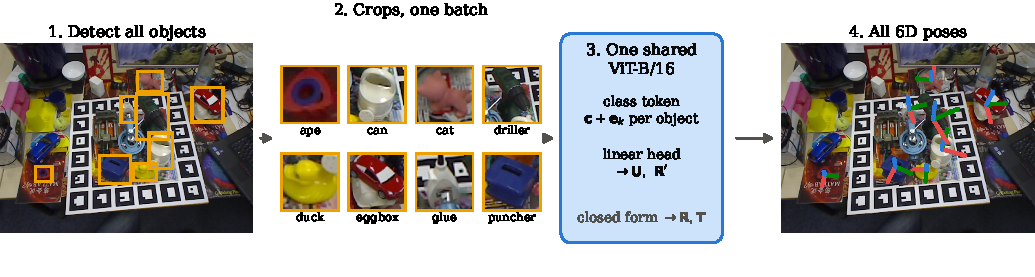
\includegraphics[width=\linewidth]{figures/teaser.pdf}
  \caption{\textbf{Overview of \ours.} (1) A detector finds every object of the dataset in the
  image; (2) each detection is cropped and all crops are processed in one batch by a single
  Vision Transformer, conditioned on the object identity by a per-object class token; (3) the
  regressed normalized translation and apparent rotation are converted in closed form into the
  full-frame pose. Real LM-O test image with the default detections and our predictions.
  \todo{First version made from real data; redraw as a clean diagram if preferred, and add the
  latency inset (\cref{fig:latency}).}}
  \label{fig:teaser}
\end{figure*}

Estimating the 3D rotation and translation (6D pose) of known objects from a single RGB image is a
key component of robotic grasping, augmented reality and autonomous inspection. The BOP
benchmark~\cite{hodan2018bop,hodan2020bop} has become the standard way to compare such methods:
it evaluates the poses of all annotated objects in real test images with the average recall (AR)
of three pose-error functions, and it encourages training on photorealistic synthetic (PBR)
images only~\cite{denninger2019blenderproc}.

The top RGB methods on BOP are \emph{hybrid}: a network predicts dense 2D--3D correspondences and
a PnP solver, usually inside RANSAC, recovers the pose~\cite{su2022zebrapose,hodan2020epos,li2019cdpn}.
Several of them train one network per object~\cite{wang2021gdrnet,liu2022gdrnpp}, and
render-and-compare methods add an iterative refinement stage~\cite{labbe2020cosypose,haugaard2022surfemb}.
These designs are accurate but expensive: the reported times on BOP range from 0.2\,s to
several seconds per image on desktop GPUs, and the number of networks grows with the number of
objects. \emph{Direct-regression} methods predict the pose with a single forward pass and are
much cheaper; recent ones close much of the gap with a single model for all objects, \eg
PViT-6D~\cite{stapf2023pvit6d} with a multi-scale ViT and PoseDETR as a single-stage detector.

FastPose-ViT~\cite{ancey2026fastposevit} showed that a Vision Transformer that directly regresses
a reformulated pose target from an object crop can be competitive with PnP-based methods for
spacecraft pose estimation, and can run in real time on an embedded Jetson device. It handles one
object, seen by one camera. In this work we ask whether the same direct-regression approach
scales to the multi-object, multi-camera setting of BOP, with one network for all objects and
synthetic training data only. To this end, we make the following contributions:
\begin{itemize}
  \item A \textbf{multi-object extension of FastPose-ViT} that keeps its simplicity: one plain
        ViT with a single linear layer, shared by all objects of a dataset and conditioned on the
        object identity by a learned per-object class token. It adds fewer than 0.05\,M
        parameters, batches the crops of different objects together, and matches eight
        single-object models trained with the same total compute.
  \item The \textbf{geometric targets for many objects and cameras}: per-image intrinsics and a
        size-invariant depth target (as in~\cite{stapf2023pvit6d}) in place of the original
        image-size-based one, which fails across objects of different sizes (+0.04 AR on LM-O),
        together with the apparent rotation, which we show remains essential on BOP (+0.11 AR).
  \item A \textbf{symmetry-aware rotation loss with translation offsets}, which takes the
        minimum over the symmetric poses of an object, including symmetries that also shift the
        object, and stays valid on the apparent-rotation targets.
  \item A \textbf{deployment study} on BOP: batched TensorRT FP16 inference with no loss in AR,
        latency as a function of the number of objects, and a multi-class LW-DETR
        detector~\cite{chen2024lwdetr} that brings the full pipeline to 55 frames per second for
        8 objects on an A100.
\end{itemize}
Trained on PBR images only, \ours{} reaches an AR of 0.668 on LM-O~\cite{brachmann2014lmo} and
0.702 on YCB-V~\cite{xiang2018posecnn} with the standard BOP detections. On YCB-V, this is the
best result among PBR-only RGB methods with one model for all objects, behind only two methods
that train one network per object; on LM-O, it is within 0.07 AR of the best PBR-only RGB methods.
\todo{Positioning to agree with the supervisor: PViT-6D (0.740) and PoseDETR (0.695) are more
accurate on LM-O.}
\pending{T-LESS result (jobs running), to add to this paragraph.}
